\documentclass{article}

\usepackage[numbers]{natbib}  % For citation management - numbers style matches current format
\usepackage{subcaption}  % Add this to preamble if not already present
\usepackage{fancyvrb}
\usepackage{amsmath,amssymb}
\usepackage{graphicx}
\usepackage{listings}
\usepackage[ruled,vlined]{algorithm2e}
\usepackage{xcolor}

% Code listing settings
\lstset{
    basicstyle=\ttfamily\small,
    breaklines=true,
    frame=single,
    numbers=left,
    numberstyle=\tiny,
    keywordstyle=\color{blue},
    commentstyle=\color{green!60!black},
    stringstyle=\color{red},
    showstringspaces=false
}
\title{Physics-Informed Machine Learning and Agent-Assisted Automation for Light Source Applications}
\author{Oliver Hoidn} % Replace with actual author name
\date{}

\usepackage[hidelinks]{hyperref}
\begin{document}
\maketitle

\section*{Introduction}
Modern light source facilities face increasingly complex operational challenges as experimental capabilities advance. At LCLS and SSRL, the combination of high data rates, sophisticated experimental controls, and growing user demand creates dual technical imperatives: the need for real-time analysis methods that maintain physical accuracy while meeting processing speed requirements, and the development of intelligent automation systems that can support both expert and non-expert users in conducting experiments efficiently.

This program proposes to address these complementary challenges through two research directions. First, the continued development of physics-informed machine learning approaches that enable real-time analysis while preserving accuracy, exemplified by the successful deployment of PtychoPINN for coherent imaging at LCLS. Second, by developing an architecture for natural language agent-assisted automation that would build on SLAC's existing beamline control and analysis systems to help users navigate data collection workflows, interpret results, and make informed decisions during beamtime.


These developments directly advance SLAC's mission of expanding scientific capabilities while enhancing facility accessibility and productivity. This research program, built on productive existing collaborations with SLAC scientists and the LCLS data analytics group, aims to improve key aspects of experimental operations and infrastructure. By addressing both computational bottlenecks and operational workflows together, this work will enable more sophisticated experiments for SLAC's expanding user community.

The two components of this program represent different stages of technical maturity with complementary risk profiles. The modeling component builds on prior success in physics-informed and probabilistic ML for lensless imaging, which I am currently developing past the proof of concept stage with collaborators at SLAC and the APS. In contrast, the AI-assisted automation framework represents a more exploratory direction that, while higher risk, offers more potentially transformative benefits. Early experiments based on a semi-automated analysis pipeline that I developed for XPP suggest significant opportunities for guidance from natural language agents to further improve beamtime efficiency. This portfolio thus combines near-term technical advances with longer-term innovation.

\section{Physics-Informed ML for Light Source Applications}
\subsection{Introduction and Challenge}
While machine learning has revolutionized many domains, the computing demands for photon science at light source facilities face unique challenges that conventional ML approaches cannot adequately address. Fast reconstruction is critical at these facilities, where experiments generate massive data streams requiring reasonably rapid analysis and feedback. Although convolutional neural networks (CNNs) excel at computer vision tasks and can offer orders-of-magnitude speedups over traditional iterative methods, their inductive biases are not aligned with physical principles. This mismatch is particularly visible in diffraction analysis, where standard neural network approaches frequently produce results that violate known physical constraints. \cite{hoidn2023physics}

\subsection{Technical Innovation - Physics-Informed ML for Imaging}
To address these limitations while preserving ML's computational advantages, I developed PtychoPINN, a physics-constrained machine learning framework for coherent diffractive imaging that combines the speed of neural networks with the accuracy of conventional optimization methods. Rather than treating reconstruction as a pure data-driven task, PtychoPINN incorporates physical constraints through a differentiable simulator that models both diffraction physics and real-space overlap conditions. This NN-simulator pipeline generates reconstructions directly from input diffraction patterns. Unlike conventional physics-informed neural networks (PINNs) that add physical constraints as regularization terms, PtychoPINN trains in a fully self-supervised fashion using a negative log likelihood loss function computed over pixels ($i, j$) and diffraction images ($k$):

\begin{equation}
\text{Loss}(x, \lambda(\hat{x})) = \sum_{i,j,k} \log f_{\text{Poiss}}(x_{ijk}^2; \lambda_{ijk})
\end{equation}


\begin{figure}[htbp]
    \centering
    \begin{subfigure}{\textwidth}
        \centering
        \includegraphics[width=0.8\textwidth]{lett.png}
        \caption{} % This adds the (A)
        \label{fig:architecture}
    \end{subfigure}
    \vspace{0.5cm}  % Vertical spacing between subfigures
    \begin{subfigure}{\textwidth}
        \centering
        \includegraphics[width=0.8\textwidth]{dose_frc50.png}
        \caption{} 
        \label{fig:efficiency}
    \end{subfigure}
  \caption{Neural network architecture and training configuration of the PtychoPINN model. (a) Schematic diagram of the physics-informed neural network architecture, showing the integration of physical constraints (real-space overlap and consistency with the forward map of far-field diffraction) with the CNN. (b) Resolution (measured by FRC50, the spatial frequency at which the Fourier ring correlation drops to 0.5) as a function of photon dose. The physically-motivated Poisson negative log-likelihood (NLL) objective function achieves the same resolution with approximately 10-fold lower dose compared to training with mean absolute error (MAE), demonstrating superior photon efficiency. }\label{diagram}
    \label{fig:combined}
\end{figure}

%\begin{figure}[h]
%\centering
%\includegraphics[width=0.9\textwidth]{lett.png}
%  \caption{Neural network architecture and training configuration of the PtychoPINN model. (a) Schematic diagram of the physics-informed neural network architecture, showing the integration of physical constraints (real-space overlap and consistency with the forward map of far-field diffraction) with the neural processing pipeline. (b) Resolution (measured by FRC50, the spatial frequency at which the Fourier ring correlation drops to 0.5) as a function of photon dose. The physically-motivated Poisson negative log-likelihood (NLL) objective function achieves the same resolution with approximately 10-fold lower dose compared to training with mean absolute error (MAE), demonstrating superior photon efficiency. }\label{diagram}
%\end{figure}

The results of this physics-first approach are compelling: PtychoPINN achieves a 4x improvement in reconstruction resolution over purely data-driven reconstruction, while being 500x faster than traditional (i.e. iterative and physics-driven) methods. It is also an order of magnitude more dose-efficient than the previous state of the art (figure \ref{diagram} (b)).

\begin{figure}[htbp]
    \centering
    \includegraphics[width=0.9\textwidth]{xpp_pinn.png}
    \caption{Comparison of conventional iterative reconstruction (left column) to physics-informed ML reconstruction (right column) and a prior state-of-the-art ML approach (center), using LCLS data (XPP, run 21). Notably -- and unlike conventional methods -- the PINN model model can reconstruct the real-space images \emph{without} ptychographic overlap information in this optical configuration.}
    \label{fig:comparison}
\end{figure}
Beyond the immediate gains in performance and throughput, this work demonstrated several principles for scientific ML: (1) physical constraints can replace the need for massive training datasets, (2) probabilistic modeling of measurement statistics significantly improves reconstruction quality at a given photon dose, and (3) physics-informed architectures lead to better generalization across different experimental conditions. The model has been validated offline on experimental data from LCLS (XPP) (ref figure) and we are currently working with APS collaborators to develop real-time reconstruction capability based on it. 

\subsection{Future Directions - Advanced Architectures for Scientific ML}
Building on PtychoPINN's foundation, I propose two technical directions that will advance our ability to handle experimental uncertainties and improve reconstruction quality:

\subsubsection{Variational Methods for Diffractive Imaging}
Probabilistic neural networks are an important development direction in scientific machine learning because they allow better modeling of stochasticities -- a special desideratum at LCLS, given the extent of shot-to-shot fluctuations -- and uncertainty quantification. PtychoPINN is currently aware of aleatoric uncertainty but lacks any estimation of epistemic uncertainties; it also neglects beam jitter. 

One of my collaborators, Aashwin Mishra (SLAC ML Initiative), has already spearheaded the development of probabilistic neural networks (PNNs) to tackle the problem of epistemic uncertainty and principled uncertainty quantification in ML models for coherent diffractive imaging. Drawing on his current efforts we plan to incorporate probabilistic techniques into PtychoPINN for improved interpretability and quantification of out-of-distribution robustness. \cite{hoidn2024probabilistic}

Furthermore, using variational autoencoders (VAEs) we could learn compact, physically meaningful representations of the complex-valued illumination in coherent imaging experiments. I propose to develop a model that jointly learns Zernike coefficients characterizing the beam illumination function jointly with phase retrieval. The VAE would provide an invertible map from the latent space to a function space of beam illumination profiles, providing a physically interpretable way to correct for shot-to-shot variation in the probe. Prior work on steerable PCA for cryo-EM has shown that such parametrizations are remarkably efficient embeddings of the illumination function. \cite{zhao2016fast}

\subsubsection{New backbone architectures for diffractive imaging}
Current neural architectures like standard CNNs lack important symmetries and properties needed for optimal performance in light source applications. I suggest new network architectures that incorporate:

Permutation invariance: Processing unordered sets of diffraction patterns necessitates models that are invariant to input ordering. By replacing standard channel-wise operations with symmetric functions that respect permutation invariance, we can design more compact and efficient architectures. This may involve creating custom convolutional kernels or employing shared-weight schemes within existing layers.

Global receptive fields through attention mechanisms: Fourier inversion problems involve long-range dependencies that are not adequately captured by local convolutional operations. Incorporating attention mechanisms into the network architecture can provide global receptive fields, enabling the model to capture all information necessary for solving the diffractive imaging inverse problem.

\subsection{Extension to Other Light Source Applications}
The above work has catalyzed productive collaborations within and beyond SLAC. At the Advanced Photon Source, Nicolas Schwarz's group is developing a PyTorch backend for PtychoPINN, while the APS Software group is working with me to incorporate it into Ptychodus, their real-time analysis framework for ptychography.

An encouraging outcome of this collaboration has been the growing interest from other national laboratories in sharing experimental data for further development. David Shapiro's group at the Advanced Light Source (ALS) has shared ptychography data, while the scientific software development group at APS has indicated they have extensive datasets that could potentially support this work. The willingness to engage reflects both interest in this research and development approach and the potential for compiling diverse experimental datasets, which will be important for generalization across different experimental configurations at various beamlines.

Such exchanges have given me a perspective on adapting prototypes to facility-specific requirements. This is a natural segue to my primary focus in this part of the research program: expanding these methods across SLAC's experimental facilities. Working with SLAC's ML Initiative and beamline scientists, I plan to identify key computational challenges where physics-informed ML can have immediate impact. The modeling principles and practical experience developed through PtychoPINN provide starting points for tackling inverse problems more generally -- especially in computed imaging, where there is a shared underlying structure between superficially disparate modalities like, for example, cryo-EM and x-ray CDI. We expect the interest in ptychography at SLAC to increase when LCLS-II-HE comes online, so now is a good time to be laying the groundwork for such efforts. 

\section{Intelligent Automation for Scientific Workflows}
Scientific facilities like SLAC face a key challenge: as experimental capabilities grow more sophisticated, the complexity of data analysis and decision-making increases dramatically. Modern AI systems, particularly Large Language Models (LLMs), offer promising capabilities for automation and assistance but face fundamental limitations when applied to demanding scientific workflows.

This section of the research program proposes a novel approach inspired by classical ideas from programming language implementation, particularly the metacircular evaluator concept from Lisp and the staged compilation techniques from modern compilers. I will argue that the LLM should be treated as a basic component of a larger system that can, if built in a certain way, be much more capable than the underlying LLM. 

If successful, the system would provide a foundation for better AI-assisted scientific workflows, enabling more aggressive automation efforts across SLAC's experimental facilities. The resulting research innovations might also give compounding returns by encouraging collaboration with the broader AI / ML research.

%\subsection{Current State and Limitations}
%Current approaches to ML-based agents in scientific settings typically focus on narrow, specialized tasks or attempt to use general-purpose LLMs as conversational assistants. While valuable, the latter tools hit fundamental barriers when faced with:
%\begin{itemize}
%    \item Reasoning requiring coherence over a series of many steps
%    \item Large inputs that exceed model context limits
%    \item Workflows needing reproducible, verifiable results
%\end{itemize}
%
%Traditional agent frameworks and tool-use architectures provide partial solutions but lack structured approaches to task decomposition and context management. They often rely on ad-hoc combinations of prompting techniques and external tools, leading to brittle solutions that scale poorly.

\subsection{Example: LLM-Assisted Analysis at XPP}
In the last year, I developed an automated analysis pipeline for LCLS's X-ray Pump-Probe (XPP) instrument, working with my PI (Apurva Mehta) and the LCLS analytics group. The pipeline (figure \ref{pipeline}) finds CDW signals through a contrast-enhancing transformation of the raw data and uses statistical criteria to maximize signal to noise with respect to the analysis parameters.


\begin{figure}[htbp]
    \centering
    % First row
    \begin{subfigure}{0.45\textwidth}
        \centering
        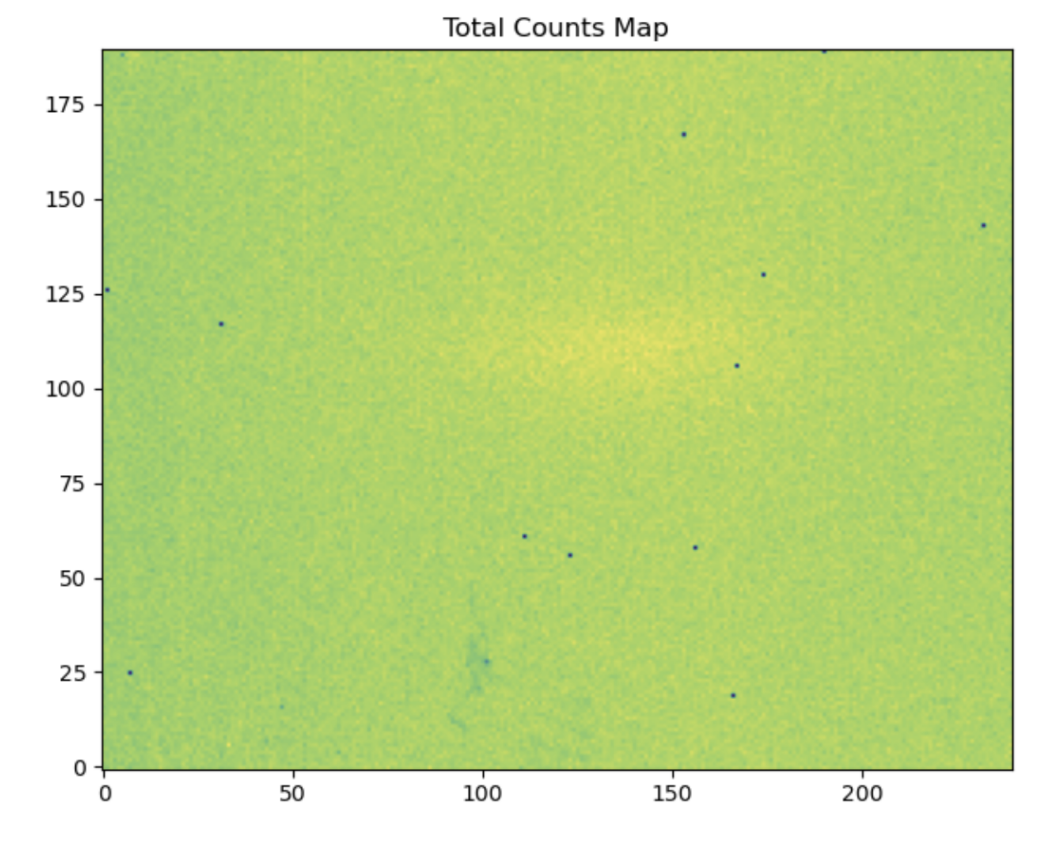
\includegraphics[width=\textwidth]{raw.png}
        \caption{}
        \label{fig:raw}
    \end{subfigure}
    \hfill  % Add horizontal space between subfigures
    \begin{subfigure}{0.45\textwidth}
        \centering
        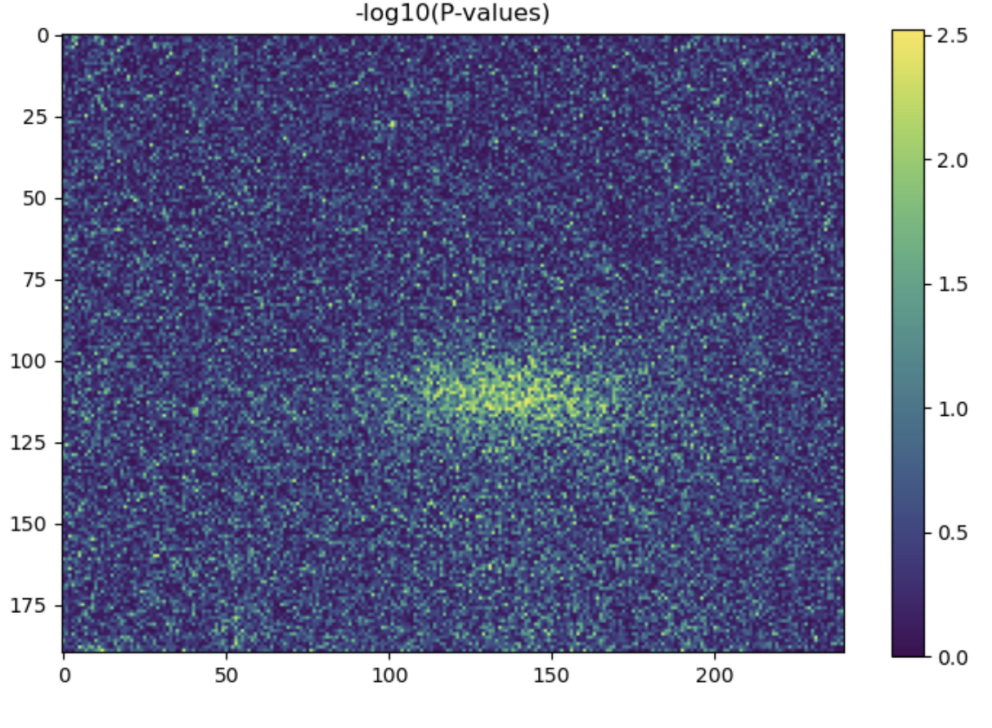
\includegraphics[width=\textwidth]{highcontrast.png}
        \caption{}
        \label{fig:highcontrast}
    \end{subfigure}
    
    \vspace{0.5cm}  % Vertical spacing between rows
    
    % Second row
    \begin{subfigure}{0.45\textwidth}
        \centering
        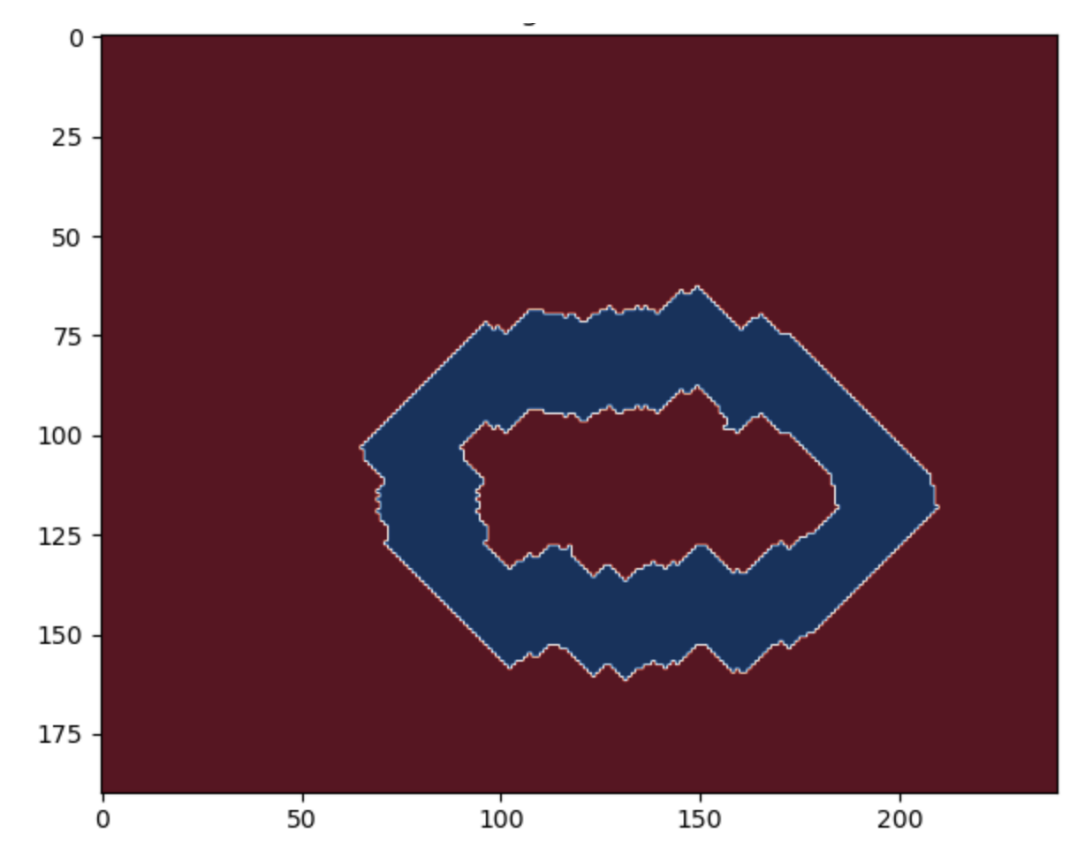
\includegraphics[width=\textwidth]{mask.png}
        \caption{}
        \label{fig:mask}
    \end{subfigure}
    \hfill  % Add horizontal space between subfigures
    \begin{subfigure}{0.45\textwidth}
        \centering
        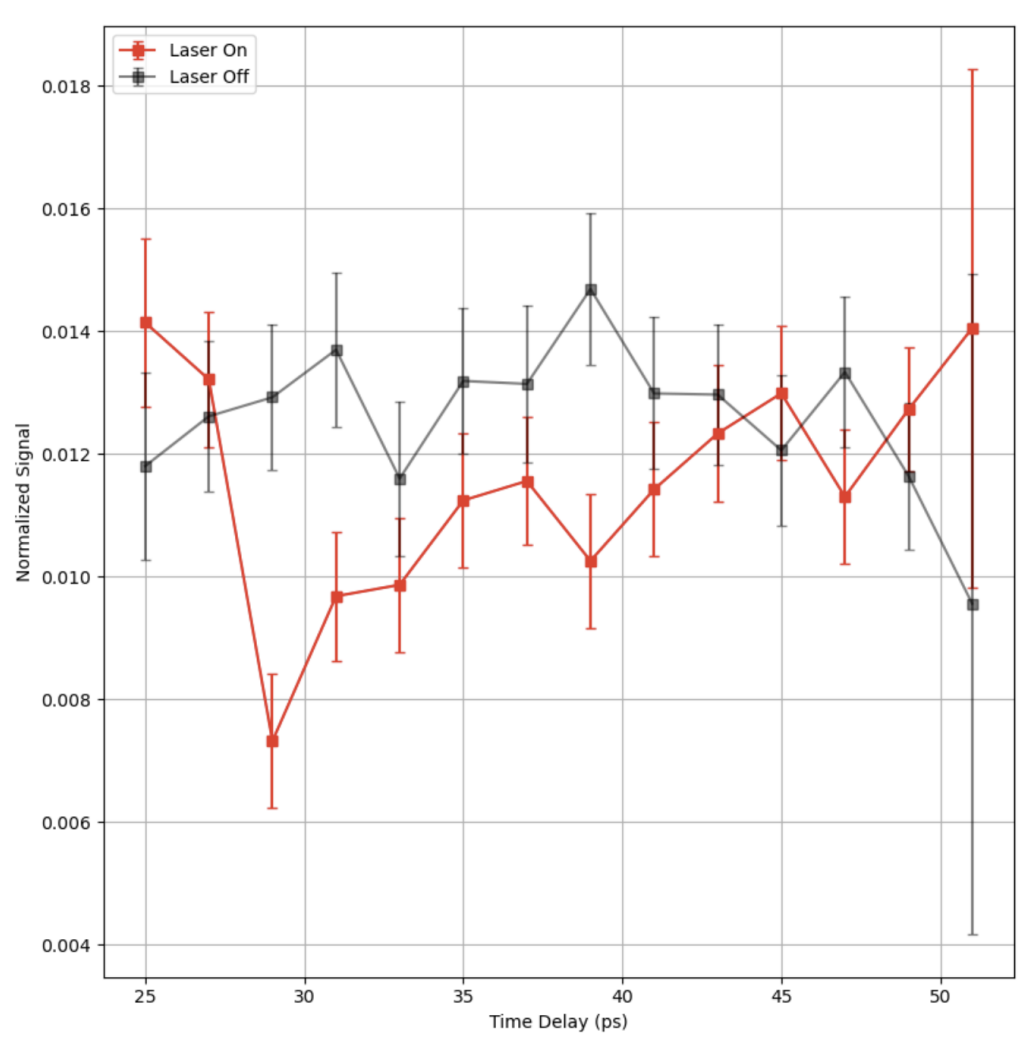
\includegraphics[width=\textwidth]{delaycurves.png}
        \caption{}
        \label{fig:delaycurves}
    \end{subfigure}
    
    \caption{In low signal-to-background settings background estimation is nontrivial, as is identifying and integrating diffraction peaks (a). Our automated workflow enhances contrast using spectral distribution statistics (b), identifies a bounding mask for the signal ((c), interior red region), estimates background levels, and finally generates a pump-probe delay curve (d). Automatic optimization of the workflow parameters yields better signal to noise than the traditional (manual) analysis.}\label{pipeline}
    \label{fig:analysis}
\end{figure}
This automation approach reduces the user's responsibility to a single numerical input: a region of interest (ROI) on the detector. While this usage is simple, interpreting diagnostic outputs when things go wrong still requires domain expertise. To address this limitation, I experimented with a language model agent to guide users through the diagnostics. In one test, I initialized the analysis with incorrect ROI coordinates. The agent reviewed logged diagnostics and successfully identified the issue:

    \vspace{0.3cm}
    \begin{Verbatim}[fontsize=\small,frame=single]
User: The pump-probe curve for the current run looks weird. What might
be wrong?

Agent: Based on the p-value uniformity check results, the designated 
background ROI [80, 95, 5, 45] appears to contain signal when it should 
not.                                                                    
This is evidenced by:

 1 Mean p-value of 0.394 (should be 0.5)
 2 Highly significant KS test (p=6.496e-17)
 3 Large z-score deviation (9.0)

This contaminated background ROI would affect the null distribution     
calculation, which in turn would distort the pump-probe curve. The      
solution would be to select a different background ROI location that    
shows proper uniformity in its p-values.
    \end{Verbatim}


While effective for modest diagnostic tasks, the system revealed fundamental limitations in more difficult situations. Attempting to use it for analyzing large collections of log files or guiding multi-step decision processes exposed a well-known underlying limitation of LLMs: difficulty maintaining analytical context across multiple interaction turns, especially when handling large datasets. This limitation is exacerbated by how LLMs perform reasoning itself - since techniques like reflection and chain of thought demonstrate that LLM `thought' operates through token generation, each step of analysis consumes valuable context window capacity.


\section{Technical Innovation: A Language-Model Architecture for Scientific Computing}
Such limitations point to a deeper challenge: we lack supporting tools for constructing agent systems in scientific environments because the underlying kernel of a natural language agent -- the LLM itself -- is on its own insufficient. Conventional automation at light sources depends on robust software design --  similarly, we will need principled architectures for composing natural language agents into scientific workflows with sufficient scale, capability and robustness.

%Scientific computing workflows demand analytical capabilities coupled with standards for reproducibility and verification. Current language model architectures, while powerful and versatile, face fundamental limitations when applied to scientific tasks. Fixed context windows put a practical cap on the amount of analysis possible within a single LLM session, as does the gradual degradation in model performance as the context window fills with output tokens.

The last two years have seen rapid growth in LLM-based agent frameworks like AutoGPT and BabyAGI. While useful, these systems rely on ad-hoc combinations of prompts and tools, making them brittle, inconsistent and hard to extend. Rather than systematically addressing the key limitations of LLMs, these agentic approaches reproduce or even compound them. A case in point is reliance on techniques such as retrieval-augmented generation (RAG) that aim to compensate for limited context window capacities but introduce serious tradeoffs in recall and accuracy.

I suggest an alternative that takes inspiration from two fundamental concepts in programming language implementation: the metacircular evaluator pattern first developed for Lisp, and staged computation techniques used in modern compilers.

The main insight is treating natural language interaction with an LLM as a form of code execution. Suppose that we first ask the LLM to translate natural language instructions into programs written in a DSL (domain specific language). The structure of such a DSL program will represent the decomposition of a complex prompt into multiple tasks. The interpretation of the same program involves distribution of each component task to an LLM instance and the linking together of instances through a calling convention and shared memory system.

More concretely:

\begin{algorithm}[H]
\SetAlgoLined
\SetKwInOut{Input}{Input}
\SetKwInOut{Output}{Output}
Natural Language Query\;
$\downarrow$ [LLM Translation]\;
XML Task Structure (equivalent to S-expression)\;
$\downarrow$ [Parser]\;
Abstract Syntax Tree\;
$\downarrow$ [tree traversal]\;
LLM execution\;
\caption{System Overview}
\end{algorithm}

In this schema, natural language queries are first translated into composite expressions made up of smaller units (atomic tasks) with the purpose to make the execution tractable while preserving semantics of the original query. A satisfying feature of the setup is that it will be self-hosting in the sense that the LLM evaluates DSL procedures generated by the LLM.

The architecture consists of three main components:

\subsection{Execution Model}
Two mutually recursive procedures, eval and apply, work with each other to evaluate DSL expressions:

\begin{lstlisting}[language=Python, caption=Core Evaluation Functions]
def EVAL(task, env):
    if primitive?(task):
        try:
            return APPLY(task, env)
        except ResourceLimit:
            new_proc = decompose(task)
            return EVAL(new_proc, env)
    else:
        # Compound task
        proc = task.procedure
        args = task.arguments
        return APPLY(proc, [EVAL(arg, env) for arg in args])

def APPLY(proc, args):
    if primitive?(proc):
        try:
            return execute_llm(proc, args)  # Direct LLM execution
        except ResourceLimit:
            # Generate new compound procedure
            new_proc = decompose(proc, args)
            return EVAL(new_proc, generate_context(proc, args))
    else:
        # Compound procedure application
        new_context = generate_context(proc.requirements, args)
        return EVAL(proc.body, new_context)
\end{lstlisting}

When task execution ends with an error (e.g. context window overrun, output validation failure), the executor can retry by generating and evaluating an alternate procedure -- for example, a decomposition of the task into multiple subtasks.

The creation of the execution data context 'env' is mediated by the memory subsystem.

\subsection{Associative memory system}
The memory system explicitly separates storage and working contexts through a hierarchical design:
\begin{itemize}
    \item Long-term memory for data and procedures
    \item Working memory for active computations
    \item Context frames that capture execution environments (including working memory)
\end{itemize}

Working memory is instantiated from long-term storage using an associative retrieval mechanism that is itself an (atomic) LLM procedure whose purpose is to match an atomic task to a contextually relevant subset of the data in long-term memory.

\subsection{Task Expression Framework}
The expression system supports nested procedures and basic functional patterns:

\begin{lstlisting}[caption=Task Expression Types]
AtomicTask     -> Direct LLM execution
NestedTask     -> Compositional evaluation  
MapExpression  -> Parallel processing
ReduceExpression -> Result combination
\end{lstlisting}

These expressions, which can be extended, provide formal semantics for the DSL.

\section{Implementation Plan}
The implementation strategy builds on recent work and collaborations at SLAC. Working with LCLS beamline scientist Lingjia Liu and Frederic Poitevin from the LCLS analytics group, I developed the previously mentioned analysis approach for charge density wave dynamics in pump-probe experiments. The project aligns with broader LCLS initiatives, led by Jana Thayer and others, to develop real-time analysis capabilities for experimental beamlines.

Building on these experiences and collaborations, the implementation will proceed in two phases:

First, we will develop the core architectural components: the memory system for managing analysis contexts, the execution model for task decomposition, and initial task libraries. These libraries will include specialized agents for software architecture, code generation, analysis refinement, and experimental log interpretation. We'll work with the LCLS analytics group to ensure the framework complements their efforts, and with beamline scientists to get feedback from the end-user point of view.

Second, we will focus on development across scientific workflows based on reusable task patterns that combine automated processing with human-in-the-loop guidance. The framework will support diverse needs, from real-time experiment optimization to offline analysis and documentation. The goals will include accelerated analysis turnaround and reduced downtime during beamtimes.

\section{Conclusion}
This research program advances two complementary directions in light source science. The first develops physics-informed machine learning for real-time analysis at light sources, demonstrated through new imaging methods that combine neural networks with physical constraints. The second proposes systematic architectures for AI-assisted tasks ranging from experimental automation to software development, drawing on principles from programming language design to address current limitations in large language models.

I worked with SLAC ML Initiative researchers to develop a physics-informed neural network approach for coherent imaging that outperforms traditional phase retrieval in speed and surpasses existing machine learning methods in resolution. Collaborators at the Advanced Photon Source (APS) and LBL are adopting these methods based on this work. In the process, I mentored an APS postdoc in extending the framework, gaining valuable experience in collaborative development that will transfer to future work at SLAC. Initial experiments with agent assistance for analysis at LCLS's XPP endstation have shown promise and illuminated key technical challenges that the proposed architectural approach aims to address.

My background prepares me to execute this research program. Through developing practical scientific machine learning methods and collaborating with a diverse group of beamline, data, and machine learning scientists, I have gained direct experience with the technical and operational challenges of light source experiments. As experimental complexity and data rates increase with the advent of LCLS-2-HE, this research aims to help SLAC meet future demands through computational advances that will enable faster analysis, more interpretable models, better-guided experiments, and overall more efficient use of facility resources. I also look forward to contributing to SLAC's educational mission by promoting the adoption of computational methods across beamlines and mentoring students and postdocs.

\section{Project links}
\begin{itemize}
\item \url{https://github.com/hoidn/PtychoPINN}
\item \url{https://github.com/hoidn/btx/tree/experiments/btx/processing/xpp}
\end{itemize}

\bibliographystyle{unsrt}  % Matches current numbering style
\bibliography{research}  % To match your filename

\end{document}

